\documentclass[a4paper]{article}
\usepackage[english]{babel}
\usepackage[utf8]{inputenc}
\usepackage{graphicx}
\usepackage{enumitem}
\usepackage{blindtext}

\usepackage{multicol}

\graphicspath{ {./images/} }
\setlength\parindent{0pt}

\title{CS2200 Homework 5}
\author{Evan Wilcox}
\date{Due April 2, 2019}

\begin{document}
  \maketitle

  \begin{enumerate}
  
  
    \item Find a deterministic finite-state automaton that recognizes the language, 
    L, consisting of all strings in \{a, b\}* that contain an odd number of b’s
    such that there is at least one a between every two b’s in the string.
    \begin{center}
      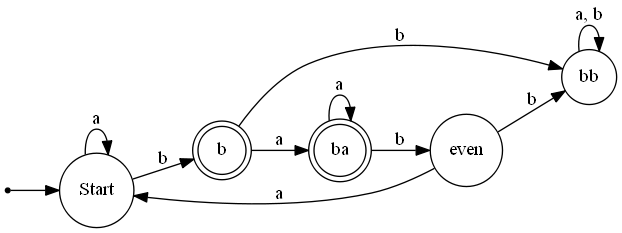
\includegraphics[scale=0.45]{1} \\
    \end{center}

    \textbf{File:} prob1.ndfsa

    \begin{multicols}{2}
    \begin{verbatim}
  A ab
  S start, 0
  S b, 1
  S ba, 1
  S bb, 0
  S even, 0
  B start
  D start, a, start
  D start, b, b
  D b, a, ba
  D b, b, bb
  D bb, a, bb
  D bb, b, bb
  D ba, a, ba
  D ba, b, even
  D even, a, start
  D even, b, bb
  T a
  O Rejected
  T b
  O Accepted
  T ab
  O Accepted
  T ba
  O Accepted
  T aba
  O Accepted
  T bab
  O Rejected
  T abaaaaba
  O Rejected
  T baaaaababa
  O Accepted
  T bb
  O Rejected
  T abbabbaba
  O Rejected
    \end{verbatim}
    \end{multicols}

    \newpage
    \textbf{File:} prob1.gv

    \begin{verbatim}
  digraph finite_state_machine {
    rankdir=LR;
    _ize="8,5"
  
    node [shape = point] x
    node [shape = circle] Start
    node [shape = doublecircle] b
    node [shape = doublecircle] ba
    node [shape = circle] bb
    node [shape = circle] even
  
    x -> Start
    Start -> Start [label = "a"]
    Start -> b [label = "b"]
    b -> ba [label = "a"]
    b -> bb [label = "b"]
    ba -> ba [label = "a"]
    ba -> even  [label = "b"]
    even -> Start [label = "a"]
    even -> bb  [label = "b"]
    bb -> bb [label = "a, b"]
  }
    \end{verbatim}

    \item Construct a regular expression that generates the language, L, defined
    in Problem 1.
    $$L = a^{*}  b  ((aa^{*}b)(aa^{*}b))^{*}   a^{*}$$

    \vspace{1cm}

    \item  Let $A = \{c,d\}$. Let $L_{2} \subseteq A^{*}$ be the language consisting 
    of all strings not in the language, $L_{3}$, which is generated by the regular 
    expression $c^{*}d^{*}c^{*}$. Find a deterministic finite-state automaton that recognizes 
    $L_{2}$.
    \begin{center}
      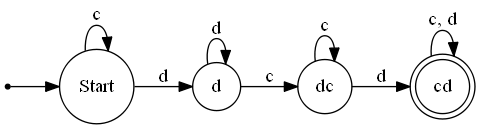
\includegraphics[scale=0.5]{3} \\
    \end{center}

    \newpage
    \textbf{File:} prob3.ndfsa
    \begin{multicols}{2}
    \begin{verbatim}
  A cd
  S Start, 0
  S d, 0
  S dc, 0
  S cd, 1
  B Start
  D Start, c, Start
  D Start, d, d
  D d, c, dc
  D d, d, d
  D dc, c, dc
  D dc, d, cd
  D cd, c, cd
  D cd, d, cd
  T 
  O Rejected
  T c
  O Rejected
  T dc
  O Rejected
  T cdc
  O Rejected
  T cccccdddddccccc
  O Rejected
  T ccccdddddccccddddd
  O Accepted
  T cdcdcdc
  O Accepted
  T dddccdcdccddcdcdcdcdc
  O Accepted
  T ccccccddddddddccccccddddddddcccccccddddd
  O Accepted
  T dddddcdcdcdcdcdddddddddccccccccc
  O Accepted 
    \end{verbatim}
    \end{multicols}

    \textbf{File:} prob3.gv
    \begin{verbatim}
  digraph finite_state_machine {
   rankdir=LR;
   _ize="8,5"

   node [shape = point] x
   node [shape = circle] Start
   node [shape = circle] d
   node [shape = circle] dc
   node [shape = doublecircle] cd

   x -> Start
   Start -> Start [label = "c"]
   Start -> d [label = "d"]
   d -> dc [label = "c"]
   d -> d [label = "d"]
   dc -> dc [label = "c"]
   dc -> cd [label = "d"]
   cd -> cd [label = "c, d"]
  }
    \end{verbatim}


    \item Find a regular expression that generates the language, $L_{2}$, defined in
    Problem 3.
    $$L_{2} = c^{*}dd^{*}cc^{*}d(c+d)^{*}$$

    \newpage
    \item Let $L_{3} \subseteq \{f, g\}^{*}$ be the language of all strings generated 
    by 
    the regular expression $(fg + ffg + fgf)^{*}$. Construct a 
    non-deterministic finite-state machine that recognizes $L_{3}$. 
    \begin{center}
      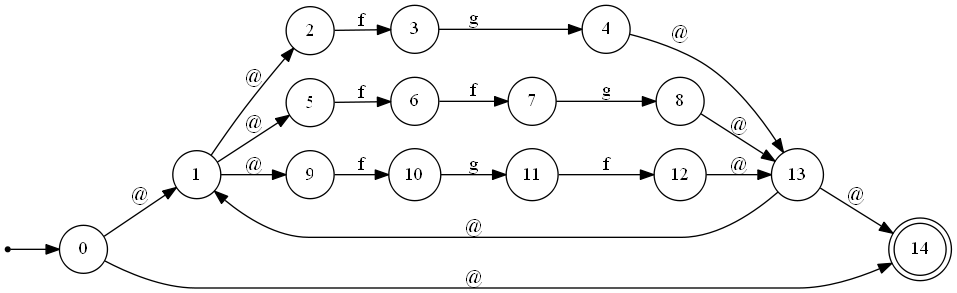
\includegraphics[scale=0.4]{5} \\
    \end{center}

    \textbf{File:} prob5.ndfsa
    \begin{multicols}{2}
    \begin{verbatim}
  A fg
  S 0, 0
  S 1, 0
  S 2, 0
  S 3, 0
  S 4, 0
  S 5, 0
  S 6, 0
  S 7, 0
  S 8, 0
  S 9, 0
  S 10, 0
  S 11, 0
  S 12, 0
  S 13, 0
  S 14, 1
  B 0
  D 0, @, 1
  D 0, @, 14
  D 1, @, 2
  D 1, @, 5
  D 1, @, 9
  D 2, f, 3
  D 3, g, 4
  D 4, @, 13
  D 5, f, 6
  D 6, f, 7
  D 7, g, 8
  D 8, @, 13
  D 9, f, 10
  D 10, g, 11
  D 11, f, 12
  D 12, @, 13
  D 13, @, 1
  D 13, @, 14
  T 
  O Accepted
  T f
  O Rejected
  T g
  O Rejected
  T fg
  O Accepted
  T ffg
  O Accepted
  T fgf
  O Accepted
  T fgffgfgffg
  O Accepted
  T ffggffg
  O Rejected
  T ffgfggfgf
  O Rejected
  T fgfgfffg
  O Accepted
    \end{verbatim}
    \end{multicols}

    \newpage
    \textbf{File:} prob5.gv
    \begin{verbatim}
  digraph finite_state_machine {
    rankdir=LR;
    _ize="8,5"
  
    node [shape = point] x
    node [shape = circle] 0
    node [shape = circle] 1
    node [shape = circle] 2
    node [shape = circle] 3
    node [shape = circle] 4
    node [shape = circle] 5
    node [shape = circle] 6
    node [shape = circle] 7
    node [shape = circle] 8
    node [shape = circle] 9
    node [shape = circle] 10
    node [shape = circle] 11
    node [shape = circle] 12
    node [shape = circle] 13
    node [shape = doublecircle] 14
  
    x -> 0
    0 -> 1 [label = "@"]
    0 -> 14 [label = "@"]
    1 -> 2 [label = "@"]
    1 -> 5 [label = "@"]
    1 -> 9 [label = "@"]
    2 -> 3 [label = "f"]
    3 -> 4 [label = "g"]
    4 -> 13 [label = "@"]
    5 -> 6 [label = "f"]
    6 -> 7 [label = "f"]
    7 -> 8 [label = "g"]
    8 -> 13 [label = "@"]
    9 -> 10 [label = "f"]
    10 -> 11 [label = "g"]
    11 -> 12 [label = "f"]
    12 -> 13 [label = "@"]
    13 -> 1 [label = "@"]
    13 -> 14 [label = "@"]
  }
    \end{verbatim}

    \newpage
    \item Using the subset construction described in class, construct a 
    deterministic finite-state machine based on the non-deterministic finite-state 
    machine that you constructed in Problem 5.
        \begin{center}
      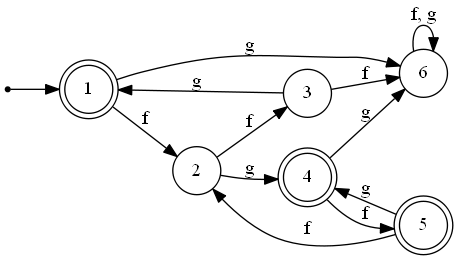
\includegraphics[scale=0.5]{6} \\
    \end{center}

    \textbf{File:} prob6.ndfsa
    \begin{multicols}{2}
    \begin{verbatim}
  A fg
  S 1, 1
  S 2, 0
  S 3, 0
  S 4, 1
  S 5, 1
  S 6, 0
  B 1
  D 1, f, 2
  D 1, g, 6
  D 2, f, 3
  D 2, g, 4
  D 3, f, 6
  D 3, g, 1
  D 4, f, 5
  D 4, g, 6
  D 5, f, 2
  D 5, g, 4
  D 6, f, 6
  D 6, g, 6
  T 
  O Accepted
  T f
  O Rejected
  T g
  O Rejected
  T fg
  O Accepted
  T ffg
  O Accepted
  T fgf
  O Accepted
  T ffggfgf
  O Rejected
  T fgfgf
  O Accepted
  T ffgfggfgf
  O Rejected
  T fgfgfffg
  O Accepted
    \end{verbatim}
    \end{multicols}

    \newpage
    \textbf{File:} prob6.gv
    \begin{verbatim}
  digraph finite_state_machine {
    rankdir=LR;
    _ize="8,5"
  
    node [shape = point] x
    node [shape = doublecircle] 1
    node [shape = circle] 2
    node [shape = circle] 3
    node [shape = doublecircle] 4
    node [shape = doublecircle] 5
    node [shape = circle] 6
  
    x -> 1
    1 -> 2 [label = "f"]
    1 -> 6 [label = "g"]
    2 -> 3 [label = "f"]
    2 -> 4 [label = "g"]
    3 -> 6 [label = "f"]
    3 -> 1 [label = "g"]
    4 -> 5 [label = "f"]
    4 -> 6 [label = "g"]
    5 -> 2 [label = "f"]
    5 -> 4 [label = "g"]
    6 -> 6 [label = "f, g"]
  }
    \end{verbatim}


    \item Let $G$ be the context-free grammar $\{ \{Q,V\}, \{c,d\},\{ Q \rightarrow QQ|V ,
    V \rightarrow cV d|cd \}, Q\}$.
    \begin{enumerate}

      \item Describe the language $L_{6} = L(G)$. Prove that $G$ is ambiguous.
    

      \item  Give an unambiguous grammar $H$, such that $L(H) = L(G)$. Give
      some justification for the claim that $H$ is unambiguous.

    \end{enumerate}

    \newpage
    \item  Consider the CFG $G = \{ \{S\}, \{a, b\}, \{S \rightarrow aSbS|bSaS|\epsilon \}, S \}$. 
    Prove by induction that $L(G) = \{ w \in \{ a, b\}^{*} |$ the number of a’s in 
    $w$ = the number of
    $b$’s in $w \}$.

    Proof 1 
    \begin{enumerate}

      \item \textbf{Define the problem.} \\
      Prove that a string generated by the CFG $G = \{ \{S\}, \{a, b\}, \{S \rightarrow aSbS|bSaS|\epsilon \}, S \}$
      has the same number of a's as it does b's.

      \item \textbf{Base case and two more.} \\
      The base case for this CFG would be substituting the empty string $\epsilon$ 
      for $S$. In the empty string there is an equal amount of a's and b's, both zero.
      When you substitute $S$ for $aSbS$ then substitute the remaining $S$'s for the 
      empty string you end up with the string 'ab' which contains an equal amount of a's
      and b's. If you substitute $S$ for $bSaS$ then substitute the remaining $S$'s with
      the empty string you get the string 'ba' which has an equal amount of a's and b's.

      \item \textbf{Inductive case.} \\
      When you substitute $S$ you have three options: $aSbS$ which adds 1 a and 1 b to 
      the string, $bSaS$ which adds 1 a and 1 b to the string, and the empty string 
      which adds no a's or b's. Because its not possible to add an a without a b or 
      a b without an a when substituting $S$, the amount of a's and b's in the string 
      will always be equal.

      \item \textbf{Conclusion.} \\
      After showing the previous two steps, we can conclude that strings generated byt the CFG 
      $G = \{ \{S\}, \{a, b\}, \{S \rightarrow aSbS|bSaS|\epsilon \}, S \}$ will have 
      equal amounts of a's and b's.

    \end{enumerate}

    Proof 2
    \begin{enumerate}

      \item \textbf{Define the problem.} \\
      Prove that a string made of a's and b's that has an equal number of a's and b's 
      can be generated by the CFG $G = \{ \{S\}, \{a, b\}, \{S \rightarrow aSbS|bSaS|\epsilon \}, S \}$.

      \item \textbf{Base case and two more.} \\
      The base case would be to generate the empty string. The empty string contains 
      an equal amount of a's and b's and can be generated directly be $S$. To generate
      the string 'ab' you can substitute $S$ for $aSbS$ then substitute $S$ for the
      empty string. To generate the string 'abab' you must substitute $S$ for $aSbS$
      then substitute the first $S$ for $bSaS$ and substitute the remaining $S$'s for 
      empty strings.

      \item \textbf{Inductive case.} \\
      The CFG's rules allows you to create every permutation of a string made of a's and 
      b's that contain an equal mount of a's and b's. The rules also allow you to chain
      these permutations.

      \item \textbf{Conclusion.} \\
      After showing the previous two steps we can conclude that all strings made of
      a's and b's containing the same amount of a's and b's can be generated by the
      CFG $G = \{ \{S\}, \{a, b\}, \{S \rightarrow aSbS|bSaS|\epsilon \}, S \}$.

    \end{enumerate}
    
    \newpage
    \item Let G be a CFG as described. Using the algorithms discussed in class, 
    convert G into an equivalent grammar that is in Chomsky Normal Form. \\

    Vars = $\{ A, B, C, D, E, F, G, H, I, J, P, Q, R, S, T, U. V. W. X, Y, Z \}$. \\
    Alph = $\{ a, b, c \}$. \\
    Start = $S$. \\
    Rules = \\
    $S \rightarrow AD|YE|UF|UG|PH|AX|YB|PQ|BZ|WC|AT|a|BT|b|UC|c|UB$ \\
    $P \rightarrow AT|a$ \\
    $Q \rightarrow QT|AQ$ \\
    $T \rightarrow CT|c$ \\
    $U \rightarrow AU|a$ \\
    $X \rightarrow AX|a|AI|AB$ \\
    $R \rightarrow AI|AB$ \\
    $Y \rightarrow YB|b|AI|AB$ \\
    $V \rightarrow BJ|BC$ \\
    $W \rightarrow WC|c|BJ|BC$ \\
    $Z \rightarrow BZ|b|BJ|BC$ \\
    $A \rightarrow a$ \\
    $B \rightarrow b$ \\
    $C \rightarrow c$ \\
    $D \rightarrow XT$ \\
    $E \rightarrow BT$ \\
    $F \rightarrow BZ$ \\
    $G \rightarrow WC$ \\
    $H \rightarrow QT$ \\
    $I \rightarrow RB$ \\
    $J \rightarrow VC$ \\



  \end{enumerate}

\end{document}